\documentclass[a4paper,12pt,autodetect-engine,dvipdfmx]{jsarticle}

\topmargin -15mm
% \oddsidemargin 0mm
% \textwidth 140mm
\textheight 210mm

\usepackage[dvips,dvipdfmx]{graphicx}
\usepackage{amsmath}
\usepackage{amsthm}
\usepackage{amssymb}
\usepackage{latexsym}
\usepackage{fancybox}
\usepackage{bm}
\usepackage{color}
\usepackage{colortbl,array,xcolor}
\usepackage{mathtools}
\usepackage[dvipdfmx]{graphicx}
\DeclarePairedDelimiter{\abs}{\lvert}{\rvert}



% \def\RC{\rowcolor{red!30}}
% \def\GC{\rowcolor{green!30}}
% \def\GC{\indexcolor{green!30}}
% \newcolumntype{R}{>{\columncolor{red!30}}c}
% \newcolumntype{G}{>{\columncolor{green!30}}c}
% \newcolumntype{A}{>{\columncolor{green!30}}c}

\theoremstyle{definition}
\newtheorem{dfn}{定義}[section]
\newtheorem{lem}[dfn]{補題}
\newtheorem{cor}[dfn]{系}
\newtheorem{exm}[dfn]{例}
\newtheorem{exa}[dfn]{例題}
\newtheorem{thm}[dfn]{定理}
\newtheorem{for}[dfn]{公式}
\newtheorem{prp}[dfn]{命題}
\newtheorem{rem}[dfn]{注意}

\makeatletter
\renewcommand{\theequation}{%
\thesection.\arabic{equation}}
\@addtoreset{equation}{section}
\makeatother
%%%%%%%%%%%%%%プリアンブル%%%%%%%%%%%%%%

\begin{document}
%%%%%%%%%%%%%%タイトル%%%%%%%%%%%%%%%%%
\begin{center}
{\LARGE{ \bf{微分積分学入門} }}

\vspace{10mm}

{\Large{ \bf{まい.}}}
\end{center}

%%%%%%%%%%%%%%概要%%%%%%%%%%%%%%%%%%%%
\bigskip
\begin{abstract}
本資料では,高校数学までの知識を前提に,理系大学生が最初に学ぶ微分積分学の概要について述べる.なるべく平素な言葉を使うことを心がけ
厳密な定義や定理を理論的に構築するよりも雰囲気を感じ取ってもらうことを優先した.
微分と積分の話を軽く述べたあと,微分と積分を語る上で欠かせない極限について述べる.論法についても
資料に入れ,微分積分の中で特に重要かつ応用がある事項について記載する.
この資料を読んだ人たちが,微分積分学についてざっくりと雰囲気を感じ取ってもらい,
さらに勉強してみようと意欲的になってもらえたら何よりも嬉しいです.

\end{abstract}
\newpage
\tableofcontents


\newpage
%%%%%%%%%%%%%%本編%%%%%%%%%%%%%%%%%%%%
\section{微分積分学とは}
微分積分学とは,接線を求める微分と面積を求める積分に関する理論である.これらが互いに逆操作であることは定義ではなく,定理として導かれる.つまり,
高校生のときに学んだ
\begin{center}
    積分は微分の逆として定義する
\end{center}
というものは一般の数学ではあまりしない.微分も積分も各々独立に定義した上で,関数に条件をつけることでそれらが逆演算の関係であることを示すことができる.

また,微分の定義式にも登場する
\begin{center}
    極限
\end{center}
に関しては$\varepsilon$ - $\delta$論法において厳密に定義することができる.高校生で学んだ極限は,直感的でわかりやすいが厳密かと言われればそうではない.
「限りなく近づく」とはわかりやすく聞き馴染みもある言葉であるが,誰にとっての限りなくなのか,そもそも定量的ではないので本当の意味で「近い」を定義できていない.
この曖昧さを全て取り除いたものが$\varepsilon$ - $\delta$論法である.

このように数学は厳密さを求める学問ですが,
\begin{center}
    大体合ってて使えたらええやん
\end{center}
なんて声が聞こえそうですが,微分積分学は専門の数学のお話なので,専門で学んできた身として完全に蔑ろにすることはしません.
噛み砕いて説明するつもりなのでどうぞお付き合いいただければと思います.また,数学科の人たちからすると逆にあまり厳密でないお話もいくつか出てくるかもしれませんが,
これは入門的な話なんだなぁと温かい目でご覧いただければと思います.
\subsection{微分とは}
微分とは,関数のある点における接線の傾きを求める操作である.中学生や高校生のときに学んだ変化の割合や平均変化率
において「幅」を0にする極限を取ったものがいわゆる微分である.初めて高校の授業で学ぶときは接線の方程式を求める問題や,
1次近似式を使うときに学ぶ.これは今から学ぶ高校レベルを超えたものでも同様であり,関数の接空間(接線の一般化)を求めたり
関数を2,3次などで近似することができる.\footnote{無限次まで扱うことである条件を満たす一般の関数を多項式のように扱えるようになる}

\subsection{積分とは}
積分とは,関数に囲まれた図形の面積を求める操作である.高校生で学ぶ積分とは異なり,微分の逆の演算として定義しない.
微分と独立に定義し,そこから関数に条件を設けることで初めて微分の逆操作であることが示される.

本来,積分は曲線で囲まれた図形をたくさんの長方形などで近似し,その長方形たちの面積の総和
(の極限)として定義される.今から学ぶ積分についても主に図形の面積を求める操作として学ぶ.
また,面積だけでなく超体積\footnote{4次元以上の図形の体積のようなもの}を求める操作としても積分は使われる.
\subsection{微分積分とは}
つまり,微分積分学とは,高校数学では逆操作として定義されていた微分と積分を別の理論として定義し,逆操作であること
を定理として理論を再構築しそれらを用いてさまざまな応用を行う学問である.また,微分と積分の定義で使われる
極限についても$\varepsilon$ - $\delta$論法により厳密に定義し,微分積分の構築の手助けをする.

\subsection{微分積分学に必要な道具}
微分積分学に必要な道具はなんといっても「極限」である.まず,微分の定義式は
\begin{equation*}
    f'(x) = \lim_{h \to 0}\dfrac{f(x + h) - f(x)}{h}
\end{equation*}
である.積分の定義式は(詳しいことは後で書く)
\begin{equation*}
    \displaystyle \int_{a}^{b}f(x)dx = \lim_{|\Delta| \to +0}\sum_{k = 1}^{n}f(x_{k})(x_{k} - x_{k-1})
\end{equation*}
である.両者ともに極限を扱っており,微分・積分を理論から厳密に理解しようとすれば極限の習熟は避けては通れないということである.
ただ,微分や積分の定理などの証明を厳密にしようとするとどうしてもこの極限を扱わないとできないだけであり,ただ単に定理などを使えれば
良いというスタンスの人たちからすれば不要なことかもしれない.

極限とは単純には,限りなく近づくときのことを調べているのだが,この「限りなく」という言葉が直感的かつ非論理的であり
扱いが難しい.極限を真面目に見つめ直すことで見えてくる理論も多く存在するので,微分積分学を語る上で極限は外せない.
\section{極限}
さて,必要だと何度も言ってきたその極限について話を始める.現実世界では,「無限大」ということは実現できない.
しかし,数学の理論としてはそれを考えることは可能であり,様々な数学の分野において非常に重要な役割を果たす.

次のような数列を考える.
\begin{equation*}
    1,\ \dfrac{1}{2},\ \dfrac{1}{3},\ \dfrac{1}{4},\ \dfrac{1}{5},\ldots,\ \dfrac{1}{n},\ldots
\end{equation*}
つまり,自然数の逆数の数が並ぶ列を考える.このとき,$n$をずっと大きくしていけば数列はどんな値になるだろうか.
\begin{equation*}
    \dfrac{1}{100000},\ \dfrac{1}{100000000000},\ \ldots
\end{equation*}
このように分母がどんどんと大きくなると分数としては小さな数になることが確認できる.もっと$n$を大きくすると,
それはもう分数としては0にとてつもなく近い数になると予想できる.これを(ちょっと雑だが)数式で表現すると
\begin{equation*}
    \dfrac{1}{10000\cdots 000000} \fallingdotseq 0
\end{equation*}
となる.

他の例も紹介しておく.例えば,
\begin{equation*}
    1-\left(\dfrac{2}{3}\right)^{1},\ 1-\left(\dfrac{2}{3}\right)^{2},\ 1-\left(\dfrac{2}{3}\right)^{3},\ldots , 1-\left(\dfrac{2}{3}\right)^{n},\ldots
\end{equation*}
のような数列があったとき,$n$をずっと大きな数字にしていくとどうなるだろうか.例えば$n=10$とすると
$\left(\dfrac{2}{3}\right)^{10} \fallingdotseq 0.017$
となり,$n$を大きくすると$n$乗されている数字は0に近い数字になっていくことがわかる.よって,
\begin{equation*}
    1 - \left(\dfrac{2}{3}\right)^{10000\cdots 00000} \fallingdotseq 1 - 0 = 1
\end{equation*}
となる.

この雑さをなくし明確に理論として定式化されたものがいわゆる極限である.「0に近い」や「ずっと大きく」とはわかりやすく聞き馴染みもある言葉であるが
誰にとってなのかが不明瞭であり,数学の理論としては「誰が見ても」が非常に重要なので,この辺りをしっかりと
理論として詰める必要がある.ただ,いきなり大学の数学で扱う理論を学ぶと頭がショートするので,高校生で学ぶ
極限から話を始める.
\subsection{高校までの極限}
高校生が学ぶ極限について述べる.先ほどの,自然数の逆数の数列が$n$を限りなく大きくすると$\dfrac{1}{n}$が限りなく0に
近づくことを,極限の英語の頭文字「lim」を用いて
\begin{equation*}
    \lim_{n \to \infty}\dfrac{1}{n} = 0
\end{equation*}
と書く.他の例も同様で,例えば前ページの2つ目の例であれば
\begin{equation*}
    \lim_{n \to \infty}\left(1 - \left(\dfrac{2}{3}\right)^{n}\right) = 1 - 0 = 0
\end{equation*}
と書く.イメージとしてはそれぞれ,
\begin{align*}
    \dfrac{1}{\infty} &= 0,\\
    1-\left(\dfrac{2}{3}\right)^{\infty} &= 1-0=0
\end{align*}
である.$\infty$にはめちゃくちゃ大きな数字が入ったと思い,計算を進めれば良い.

一般的に数列$a_{n}$を用いて次のように定義を記述する.
\begin{dfn}
    数列$\{a_{n}\}$において,$n$を限りなく大きくしたとき,$a_{n}$が限りなく$\alpha$に近づくことを
    \begin{equation*}
        \lim_{n \to \infty}a_{n} = \alpha
    \end{equation*}
と定義する.また,このときの$\alpha$を極限値という.
\end{dfn}
上記のように,必ず極限値をもつかというとそうではない.例えば数列$a_{n}$が
\begin{equation*}
    a_{n} = n
\end{equation*}
であるとき,$n \to \infty$とすると数列がどんどんと大きくなっていくことは想像に容易いと思う.このような場合,
数列$a_{n}$の$n \to \infty$における極限値は存在しないという.
まとめると次のようになる.
\begin{dfn}
    数列$a_{n}$の極限値が存在するとき,数列$a_{n}$は
    \begin{center}
        収束する
    \end{center}
    といい,収束しない場合
    \begin{center}
        発散する\footnote{無限大になるものだけ発散すると表現をするという意見があるが,本文の定義がおそらく正しい.振動(後で記載)も正確には発散に含まれる.}
    \end{center}
    という.
\end{dfn}
数列を$a_{n} = (-1)^n$と定義すると,この数列は$1,\ -1$を交互に取り続ける数列となる.このとき,$n \to \infty$としても数列は収束しない.
この数列は発散するが,特にある特定の値を行ったり来たりするような場合,「振動する」という.
\subsection{数列の極限の例}
ここでは,簡単な数列の極限の計算例を示す.
\begin{exa}
    $a_{n} = \dfrac{2n^2 + n - 1}{n^2 - 3n +9}$のとき,$\displaystyle \lim_{n \to \infty}a_{n}$を求める.
\end{exa}
まず,そのまま数列に$\infty$を入れてみると,
$$\dfrac{\infty}{\infty}$$
となり,計算ができない.このような形は不定形と呼ばれ,適切な計算をすることで極限値を計算できる場合がある.
数列$a_{n}$を次のように計算する.
\begin{align*}
    a_{n} &= \dfrac{2n^2 + n - 1}{n^2 - 3n +9}\\
          &= \dfrac{2 + \frac{1}{n} - \frac{1}{n^2}}{1 - \frac{3}{n} + \frac{9}{n^2}}.
\end{align*}
このように計算すれば,$\dfrac{1}{n}$や$\dfrac{1}{n^2}$は$n \to \infty$のとき0になるので,
\begin{align*}
    \lim_{n \to \infty}a_{n} &= \lim_{n \to \infty}\dfrac{2 + \frac{1}{n} - \frac{1}{n^2}}{1 - \frac{3}{n} + \frac{9}{n^2}}\\
                             &= \dfrac{2 + 0 - 0}{1 - 0 + 0}\\
                             &= 2
\end{align*}
のように収束し,その極限値が2であることがわかる.
\begin{exa}
    $b_{n} = \dfrac{3n^3 + n - 2}{2n^2 - 5n +1}$のとき,$\displaystyle \lim_{n \to \infty}b_{n}$を求める.
\end{exa}
数列の分母の最高次に着目して計算すると,
\begin{align*}
    \lim_{n \to \infty}b_{n} &= \lim_{n \to \infty}\dfrac{3n + \frac{1}{n^2} - \frac{2}{n^2}}{2 - \frac{5}{n} + \frac{1}{n^2}}\\
                             &= \infty
\end{align*}
となり,この数列は無限大に発散する.
\begin{exa}
    $c_{n} = \sqrt{n^2 + n + 2} - n$のとき,$\displaystyle \lim_{n \to \infty}c_{n}$を求める.
\end{exa}
まず,そのまま数列に$\infty$を入れてみると,
$$\infty - \infty$$
となり,計算ができない.今回のものも不定形と呼ばれ,適切な計算をすることで極限値を計算できる.
\begin{align*}
    \lim_{n \to \infty}c_{n} &= \lim_{n \to \infty}\sqrt{n^2 + n + 2} - n\\
          &= \lim_{n \to \infty}\dfrac{n^2 + n + 2 - n^2}{\sqrt{n^2 + n + 2} + n}\\
          &= \lim_{n \to \infty}\dfrac{1 + \frac{2}{n}}{\sqrt{1 + \frac{1}{n} + \frac{2}{n^2}} + 1}\\
          &= \dfrac{1}{1 + 1}\\
          &= \dfrac{1}{2}
\end{align*}
このように,分子の有理化をすることで計算でき,その極限値は$\dfrac{1}{2}$となる.
\begin{exa}
    $d_{n} = \dfrac{3^{n+1} - 2 ^{n} + 1}{3^{n} + 4 \cdot 2^{n} + 4}$のとき,$\displaystyle \lim_{n \to \infty}d_{n}$を求める.
\end{exa}
分数に指数が入っていても基本的な計算方針は変わらない.分母の指数の底が最も大きい$3^n$で分母分子を割ると,
\begin{align*}
    \lim_{n \to \infty}d_{n} &= \dfrac{3 - \left(\frac{2}{3}\right)^{n} + \frac{1}{3^n}}{1 + 4\cdot \left(\frac{2}{3}\right)^{n} + \frac{4}{3 ^ n}}\\
                             &= \dfrac{3 - 0 + 0}{1 + 4\cdot 0 + 0}\\
                             &= 3
\end{align*}
と収束してその極限値は3となる.

上記の例のように,不定形で一見極限値をもたないような数列であっても,適切な計算をすることで極限値を求めることができる.
また,四則演算の極限値においては,収束する場合次のような定理がある.
\begin{thm}\label{thm.2.7}
    数列$a_{n},\ b_{n}$がそれぞれ極限値$\alpha,\ \beta$をもつとする.つまり,
    $$\lim_{n \to \infty}a_{n} = \alpha,$$
    $$\lim_{n \to \infty}b_{n} = \beta$$
    とする.このとき,次が成り立つ:
    \begin{align*}
        \lim_{n \to \infty}(a_{n} \pm b_{n}) &= \alpha \pm \beta,\\
        \lim_{n \to \infty}a_{n} \cdot b_{n} &= \alpha \beta,\\
        \lim_{n \to \infty}\dfrac{a_{n}}{b_{n}} &= \dfrac{\alpha}{\beta}\ (\beta \neq 0).
    \end{align*}
\end{thm}
つまり,収束する数列に対しては,四則演算はそのまま極限値にも引き継がれる.上記でたくさんの例を見てきたが,どの極限においても,
\begin{center}
    限りなく$n$が大きいとき,$a_{n}$は限りなく極限値$\alpha$に近づく
\end{center}
ということを述べている.つまり,
$$\lim_{n \to \infty}a_{n} = \alpha$$
というこの短い等式には多くの意味が込められていることに注意してもらいたい.

不定形については様々な形が存在するが,下記の形になっているものは不定形と呼ばれる.
\begin{align*}
    \dfrac{\infty}{\infty},\ \dfrac{0}{0},\ \infty - \infty,\ {\infty}^{0},\ {0}^{0},\ 0 \times \infty,\ 1 ^ {\infty}
\end{align*}
上記の形の場合,極限値を求めることは困難であるが,概ね計算可能な場合が多い.それぞれの不定形に対してどのようなアプローチを取れば計算が
可能になるのかは高校の教材などで学ぶと楽しめるだろう.

また,極限には上記で説明した「数列の極限」と「関数の極限」の2種類がメインだが,関数の極限の方は詳しくは書かない(そもそもこの資料の読者は高校卒業くらいの方を想定して書いているため).

高校数学における極限の定義を用いても,極限計算は十分に行うことができ,正直なところ大学の数学を本格的にしないので
あればこれ以上のものを学ぶ必要はない.また,大学数学における極限の問題においても高校数学で学ぶ直感的な極限
計算は非常に重要である.次の節では理論的な内容になるが,わからなければ飛ばしても多少は問題ないだろう.
\subsection{大学数学における数列の極限}
この節では,極限を厳密に定義することを目的とする.高校までの極限の定義では「限りなく」という(直感的だが)曖昧な
言葉が混ざっていた.この「限りなく」を数式と論理で定式化することで,極限というものを厳密に扱う.初めてこの理論に
触れる読者はかなり理解に時間を要するので,軽く読んでみて興味が出なければ飛ばしてもらっても構わない.\footnote{筆者は大学1年生の春にこの理論を学んで,ちゃんと理解して問題が解けるようになったのは1年後だった.さらに,他人に教えられるようになったのは大学3年生になる直前くらいだった.}
\subsection{$\varepsilon$ - $N$論法}
数列の極限を厳密に定式化する理論は
\begin{center}
    $\varepsilon$ - $N$論法
\end{center}
と呼ばれる.この2つの文字($\varepsilon$と$N$)を用いて,「限りなく」という言葉の曖昧さを消す.

さて,改めて高校数学における極限の定義を思いだそう.
\begin{dfn}[再]
    数列$\{a_{n}\}$において,$n$を限りなく大きくしたとき,$a_{n}$が限りなく$\alpha$に近づくことを
    \begin{equation*}
        \lim_{n \to \infty}a_{n} = \alpha
    \end{equation*}
と定義する.また,このときの$\alpha$を極限値という.
\end{dfn}
この定義に現れる「限りなく」は2つある.それは$n$を限りなく大きくするところと,$a_{n}$が限りなく$\alpha$に近づく
という2つである.意味が通じるのだから,それでいいじゃないかとも思うが,数学は誰が見ても$\dot{そ}\dot{う}\dot{だ}$と言える定義でなければならない.
高校数学の極限の定義では,「誰にとっての限りなく」なのかがはっきりとはわからない.限りなく$n$が大きいとき,と言われてもそれは
$n=100$なのか$n=10000$なのか$n=1000000000000$なのか,また,$a_{n}$が$\alpha$に近いとはそもそも何なのか,近いというと
どれくらい近いのか,などなど数学の理論としては完全に定式化されているとは言い難いものである.

では,「限りなく大きい」や「限りなく近い」を一度決めてみて定義を改めてみるが,その前に仮定と結論を再確認しておこう.
定義2.8における仮定は
\begin{center}
    $a_{n}$の$n$を限りなく大きくしたとき
\end{center}
であり,結論は
\begin{center}
    $a_{n}$が限りなく$\alpha$に近づく
\end{center}
である.さらに,抽象さを少なくし,具体的に物事議論するために以降は
$$a_{n} = \dfrac{1}{n},\ \alpha = 0$$
とする.もちろん,これから得たい結論は
$$\lim_{n \to \infty}\dfrac{1}{n} = 0$$
である.

さて,結論の「限りなく近い」ということを差の絶対値が0.01未満になると(恣意的に)定義しよう.つまり,
$$\left|\dfrac{1}{n} - 0\right| < 0.01$$
を満たすとき$\dfrac{1}{n}$は$0$に限りなく近いと定義し,これを満たしたときに
$$\lim_{n \to \infty}\dfrac{1}{n}= 0$$
と書くことにする.このように極限を定義するとき,仮定である「$n$を限りなく大きくしたとき」の$n$はどこまで大きくすればよいだろうか.
例えば,$n=10$とすると,
$$\dfrac{1}{n} = 0.1$$
となり,「限りなく近くない」ことがわかる(0との差の絶対値が0.01未満ではない).では,思い切って大きくして$n=1000$とするとどうだろうか.
このとき,
$$\dfrac{1}{n} = 0.001$$
となり,「限りなく近い」ということがわかる.よって,
\begin{center}
    $n=1000$のように$n$を大きくしたとき,$\left|\dfrac{1}{n} - 0\right| < 0.001 < 0.01$
\end{center}
が成り立つので,
$$\lim_{n \to \infty}\dfrac{1}{n}= 0$$
が証明されたことになる.あくまでこの証明は,$\dfrac{1}{n}$が0に限りなく近いという定義を差の絶対値が0.01未満になるに
なるときと定義したときだけのものであることに注意する.もしかすると,
\begin{center}
    いやいや,私の(俺の)「限りなく小さい」はもっと小さい数を使う.差の絶対値が0.0000001未満のときじゃないと$\dfrac{1}{n}$が限りなく0に近いとは言えないね
\end{center}
などと言う人がいるかもしれない.つまり,上記の人は
\begin{equation*}
    \left|\dfrac{1}{n} - 0 \right| < 0.0000001
\end{equation*}
のときに
$$\lim_{n \to \infty}\dfrac{1}{n}= 0$$
を認めると言っているのである.では,それを満たすように$n$を限りなく大きくすればよい.例えば,
$$n = 1000000000$$
と$n$を限りなく大きくすれば
$$\dfrac{1}{n} = 0.000000001$$
となり,0との差の絶対値が0.0000001未満になっているので,$\dfrac{1}{n}$が限りなく0に近いと言える.

このように,人によって結論,$\dfrac{1}{n}$が0に近いという定義が異なる.しかし,どのような近さを言われたとしても
適切に$n$を大きくすることで,その人の定義に合わせて$\dfrac{1}{n}$が0に近いということを証明することができる.これこそが,
\begin{center}
    $n$を限りなく大きくするとき,$\dfrac{1}{n}$が限りなく0に近づく
\end{center}
ことを表している.

では,どんな人がどんな「限りなく近い」の定義を持ってこようとも,適切に$n$を大きくすることでその定義に当てはまる
ようにできればよい.誰になんと言われても文句がないように,「限りなく近い」として任意に$\varepsilon > 0$を
とってくる.つまり,
$$\left|\dfrac{1}{n} - 0 \right| < \varepsilon$$
のときに
$$\lim_{n \to \infty}\dfrac{1}{n}= 0$$
が成り立つとする(この$\varepsilon$は0.000001のようなメチャクチャ小さな数と思う).このとき,どれほど$n$を
大きくすれば良いかというと,
$$n > \dfrac{1}{\varepsilon}$$
となるような自然数$n$を持ってくれば,
\begin{align*}
    \left|\dfrac{1}{n} - 0\right| &= \dfrac{1}{n}\\
                                  &< \varepsilon
\end{align*}
となり,「限りなく近い」の定義に当てはめることができる.誰かが,$\dfrac{1}{n}$が限りなく0に近いことを,
差の絶対値が$\varepsilon$未満になることと定義してきてから,その定義してきた$\varepsilon$を使って$n$を
定めるということを行っている.大事なことなのでもう一度述べておくが,この$\varepsilon$は任意なので,誰が
どんな数を言おうとこの$\varepsilon$で対応ができる.\footnote{筆者がこの$\varepsilon$について習ったとき,「クレーム対応をするために任意にする」と教えられたのはなかなか記憶に残っている}

議論を整理しよう.
$$\lim_{n \to \infty}\dfrac{1}{n} = 0$$
を証明するためにまずは,$\dfrac{1}{n}$が0に限りなく近いを任意の$\varepsilon > 0$を用いて
$$\left|\dfrac{1}{n} - 0 \right| < \varepsilon$$
によって定義した.その後,この定義に当てはまるような大きな$n$を$\varepsilon$を使って定める.誰が
どんな近い尺度を持ってきても,適切に$n$を大きくすることで(例えば$n > \frac{1}{\varepsilon}$を満たすような$n$)限りなく近いの定義に当てはめられる.よって,
$$\lim_{n \to \infty}\dfrac{1}{n} = 0$$
が成り立つ.という流れである.

このとき,注意すべきことが1つある.それは,限りなく近いの定義である
$$\left|\dfrac{1}{n} - 0 \right| < \varepsilon$$
を満たすような$n$は1つだけあればよいということではなく,とある数から全ての$n$が限りなく近いの定義に当てはまっている
必要がある.例えば次の数列を考えてみよう.
\begin{equation*}
    a_{n} = 
    \begin{cases}
        \dfrac{1}{n} & (nは10の倍数でない)\\
        1 & (nは10の倍数)
    \end{cases}
\end{equation*}
少しわかりづらい数列だが,次のグラフを見れば理解が深まると思われる(手書きですみません).

\begin{center}
    \includegraphics[width=13cm]{frac{1}{n}.jpeg}
\end{center}

さて,この数列に対して,
\begin{equation*}
    \lim_{n \to \infty}a_{n}
\end{equation*}
はどうなるだろうか.ほとんどの数の場合は大きな数$n$の逆数になり,$n$を大きくすれば0に近づくかもしれないと思うが,
定期的に数列の値が1になる部分もある.よって,この数列は収束しなさそうだと予測される(実際収束しない).どれだけ$n$を大きくしても,$\varepsilon = \dfrac{1}{2}$としてしまうと(1未満の数であればなんでも良いが)それは
$$\left|\dfrac{1}{n} - 0 \right| < \varepsilon = \dfrac{1}{2}$$
を満たさなくなってしまう.例えば,$n=100000000$という大きな数でも$a_{n}=1$となり,$\dfrac{1}{2}$をこえる.
10の倍数以外の自然数であれば限りなく近いの定義に当てはまりそうだが,あらゆる10の倍数はそうではない.
このとき$a_{n}$は$n$が十分大きいときに限りなく0に近いとは言い難い.
つまり,この数列は収束しない.

上記の$a_{n}$のように,ある$n$からすべてが「限りなく近い」の定義に当てはまっていないと収束したと
認めづらい,というか認めれらないことがわかる.よって,改めて極限の定義を練り直すと次のようになる.

任意の$\varepsilon > 0$に対して,ある自然数$N > 0$を用意したとき,$n > N$を満たすすべての$n$に対して
$$\left|\dfrac{1}{n} - 0 \right| < \varepsilon$$
を満たすとき,
$$\lim_{n \to \infty}\dfrac{1}{n} = 0$$
と表す.

この定義を一般の数列$a_{n}$や$\alpha$に置き換えることで,$\varepsilon$-$N$論法の定義が次で完成する.
抽象的なので,今後も難しいと感じたら具体的な数列や収束値に置き換えて考えるとよい.
\begin{dfn}
    任意の$\varepsilon > 0$に対して,ある自然数$N>0$が存在し,$n>N$を満たす全ての$n$に対して
    $$\left|a_{n} - \alpha\right| < \varepsilon$$
    が成り立つとき,\footnote{「$n>N$を満たす全ての自然数に対して不等式を満たす」ような自然数$N$が存在するとき,と考える.}
    $$\lim_{n \to \infty}a_{n} = \alpha$$
    と定義する.
\end{dfn}
「任意」を$\forall$,「存在」を$\exists$で表し,論理記号を用いて厳密に定義を書こうとすると,次のようになる.
\begin{equation*}
    ^{\forall}\varepsilon > 0,\ ^{\exists}N \in \mathbb{N}\ s.t.\ ^{\forall}n>N,\ \left|a_{n} - \alpha\right| < \varepsilon
\end{equation*}
ここで,「$s.t.$」はsuch thatの略で,「〜〜のような」という意味を持つ.上記の定義であれば,$s.t.$以下の条件が
成り立つような,という意味で使用される.また,$\mathbb{N}$は自然数全体の集合を表す.すなわち,
$$\mathbb{N} = \{1,2,3,4,\ldots\}$$
である.

このような論理記号の定義は「日本語」という曖昧なものから脱却し,厳密に定式化することが可能であるが,ご覧の通り
見た目がえげつないことになるので覚える必要はない.まずは定義2.9の内容を完璧にすることをお勧めする.

さて,定義2.9が書けたということは,極限等式である
$$\lim_{n \to \infty}\dfrac{1}{n} = 0$$
を証明する必要がある(できる)ということになる.では,改めた$\varepsilon$-$N$論法を用いて証明しよう.
\begin{proof}
    任意に$\varepsilon>0$をとる.このとき,自然数$N$を$N>\dfrac{1}{\varepsilon}$を満たすように,
    例えば,$N=\left[\dfrac{1}{\varepsilon}\right]+1$とする(ガウス記号)と,$n>N$を満たす任意の$n$に対して,
    \begin{align*}
        \left|\dfrac{1}{n} - 0 \right| &= \dfrac{1}{n}\\
                                       &< \dfrac{1}{N}\\
                                       &= \dfrac{1}{[\frac{1}{\varepsilon}]+1}\\
                                       &< \dfrac{1}{\frac{1}{\varepsilon}}\\
                                       &= \varepsilon
    \end{align*}
    が成り立つ\footnote{ガウス記号の性質の1つである,$[x] \leq x < [x] + 1$を用いた}.よって,
    $$\lim_{n \to \infty}\dfrac{1}{n} = 0$$
    が証明された.
\end{proof}
このように証明することができるが,やはり疑問に思うことは,
$$N = \left[\dfrac{1}{\varepsilon}\right]+1$$
がどうやって出てきたのかである.これは筆者もはじめは疑問に思ったが,これには2つ注意すべき点がある.
1つは,
\begin{center}
    別に$N = \left[\dfrac{1}{\varepsilon}\right]+1$である必要はない
\end{center}
ということである.定義2.9で述べている「存在する」とは,何か1つあればよく,それは条件を満たすものなら本当になんでも良い(が,明確に1つはバシッと決まっている必要はある).
例えば教科書の練習問題の答えとは違っていても正しい$N$を選択できている場合がある.なので,
\begin{align*}
    N &= \left[\dfrac{1}{\varepsilon}\right]+1\\
    N &= \left[\dfrac{1}{\varepsilon}\right]+2\\
    N &= \left[\dfrac{2}{\varepsilon}\right]+1
\end{align*}
のどれでも正しい回答となる.ただし,その選択した$N$から差の絶対値が$\varepsilon$で上から抑えられる\footnote{数学における業界用語であり上から評価するとも言う.$a<b$のことを$a$を上から$b$で抑えるという.}ことを
ちゃんと示す必要がある.

2つ目は
\begin{center}
    この$N$は証明とは別の場所で計算する必要がある
\end{center}
ということである.つまり,証明の清書の前の下書きの段階で求めておくということである.例えば今回の場合は,
$$\left|\dfrac{1}{n}- 0\right| < \varepsilon$$
を示せば良いとあらかじめわかっているので,
\begin{equation*}
    \dfrac{1}{n} < \varepsilon
\end{equation*}
を$n$について解いて
$$n > \dfrac{1}{\varepsilon}$$
となるように$n$を選ぶ必要があるとわかる.今回の場合はかなり簡単に$n$が求まるが,複雑な問題はもっと苦労する(けど求める感覚は次第に身につく).
そして,定義には自然数$N$を決める必要があるので,$\dfrac{1}{\varepsilon}$を超えるような自然数として,
$$N = \left[\dfrac{1}{\varepsilon}\right]+1$$
を選んだわけである.特にガウス記号は単に自然数に無理矢理変換するためのもので、どの証明にも必須というわけではない.

改めて,図を見ながらこの証明が何をやっているのか理解しよう.この論法が述べていることは
\begin{center}
    どんなに小さな誤差($\varepsilon$)を用意しても,あるところから数列と極限値の差の絶対値がその小さな誤差におさまっている
\end{center}
ということである.$\varepsilon$で上から抑えられるとは,数列のグラフが$2\varepsilon$の幅の中に
おさまっていることを表す.また,$n>N$を満たす任意の$n$とはある縦ラインから右側にあるすべての$n$を指す.
つまり,どれだけ誤差の幅を小さくしても,$N$を適切にとってくることで,それより右側にある数列$\dfrac{1}{n}$たちが全て小さな誤差
の中に入ることを意味する.

\begin{center}
    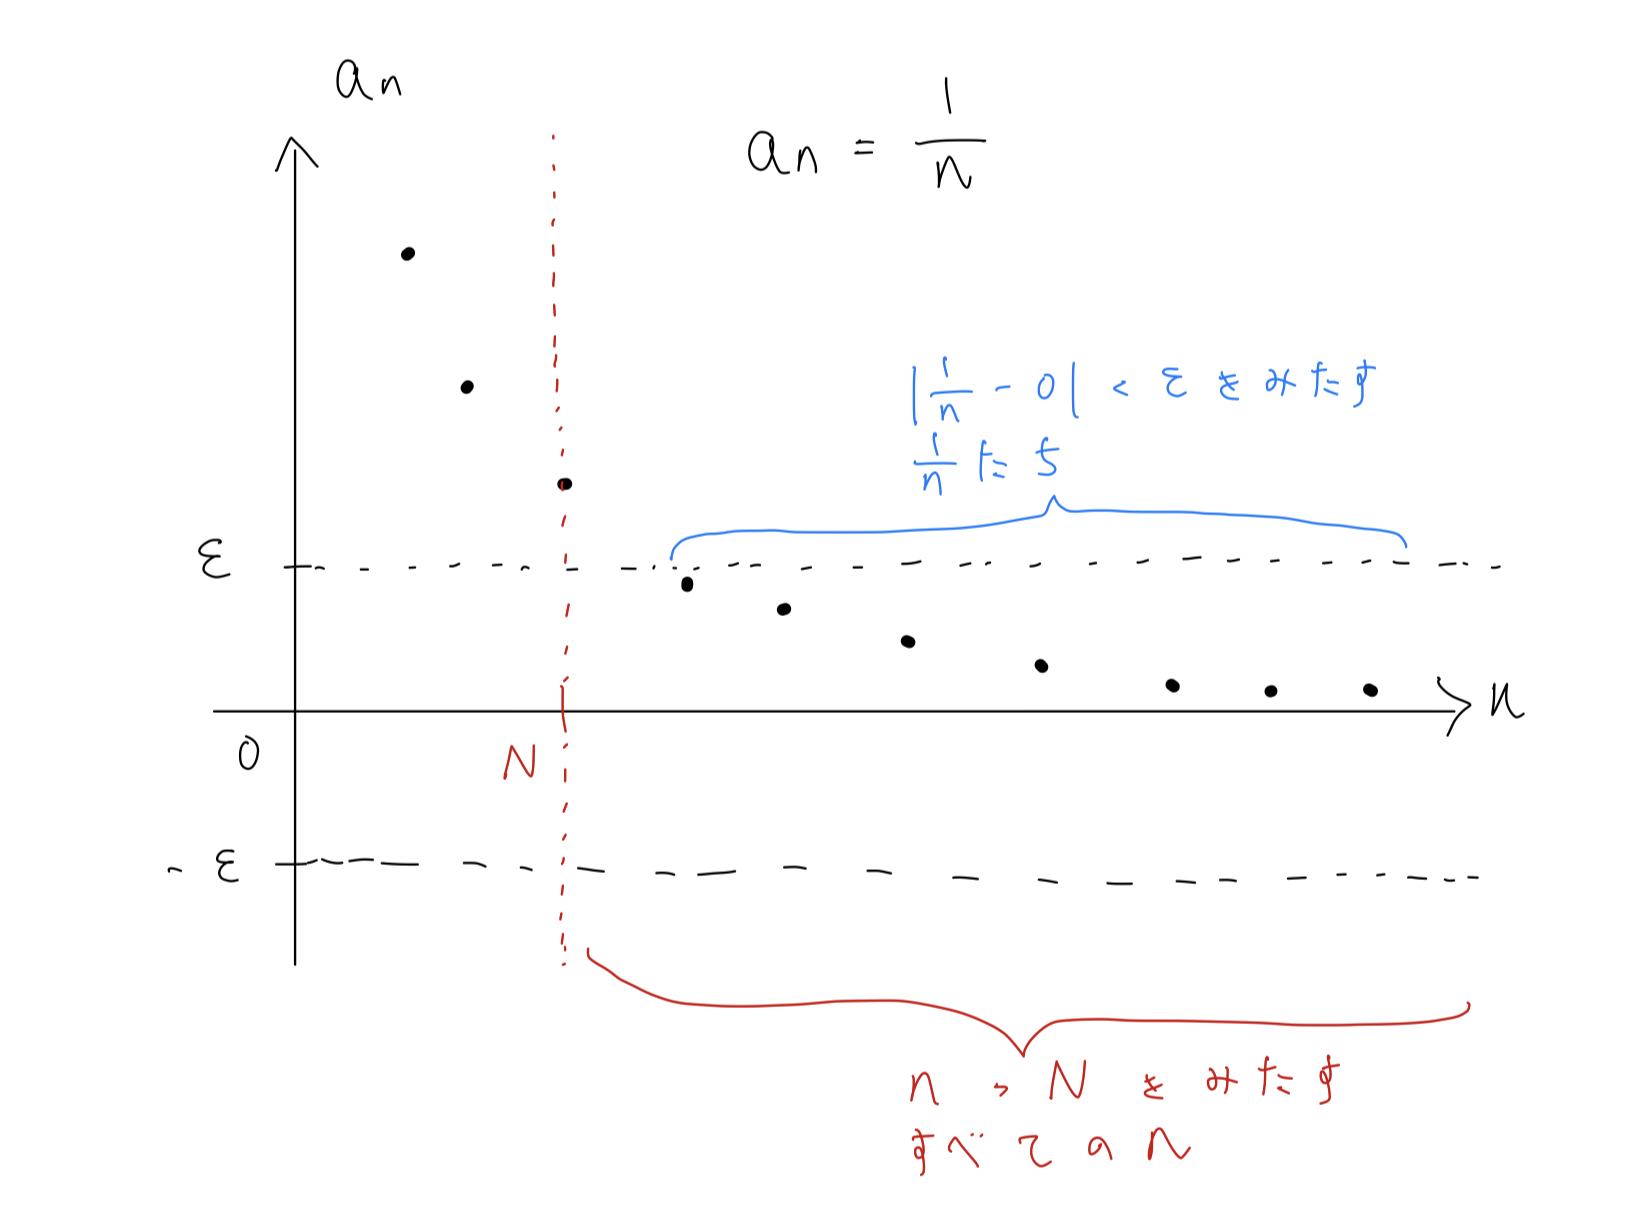
\includegraphics[width=13cm]{image.jpeg}
\end{center}
これがグラフで捉えた$\varepsilon$-$N$論法である.さまざまな観点で観察してきたが,それでもなおこの理論は
難しいと筆者は思う.たくさんの問題に触れて経験値を積んでいってほしい.

ということで,別の数列の極限の証明をする.
\begin{exa}
    $a_{n} = \dfrac{n}{n+1}$のとき
    $$\lim_{n \to \infty}a_{n} = 1$$
    を証明する.
\end{exa}
まずは予備考察として示したいことの確認と$N$を定めるための計算をする.

示したいことは任意の$\varepsilon > 0$に対して
$$\left|\dfrac{n}{n+1} - 1\right| < \varepsilon$$
である.
$N$を定めるために,上記の不等式を$n$について解く.
\begin{equation*}
    \left|\dfrac{n}{n+1} - 1\right| = \dfrac{1}{n+1}
\end{equation*}
なので,
\begin{equation*}
    n > \dfrac{1}{\varepsilon} - 1
\end{equation*}
となる.よって,この不等式の右辺の値より大きな自然数として
$$N = \left[\dfrac{1}{\varepsilon}\right]$$
を選べば良さそうである.
\begin{proof}
    任意に$\varepsilon > 0$をとる.$N=\left[\dfrac{1}{\varepsilon}\right] \in \mathbb{N}$とすると,$n>N$を
    満たす任意の$n$に対して,
    \begin{align*}
        \left|\dfrac{n}{n+1} - 1\right| &= \dfrac{1}{n+1}\\
                                        &< \dfrac{1}{N+1}\\
                                        &= \dfrac{1}{[\frac{1}{\varepsilon}] + 1}\\
                                        &\leq \dfrac{1}{\frac{1}{\varepsilon}}\\
                                        &= \varepsilon
    \end{align*}
    が成り立つ.よって,
    \begin{equation*}
        \lim_{n \to \infty}\dfrac{n}{n+1} = 1
    \end{equation*}
    が示された.
\end{proof}
このように極限等式を証明することができる.予備考察がなければ$N$の選び方が不明すぎるが,例えば試験などで解答
する場合にはそれは答案用紙に書く必要もない(だって証明ができているのだから).任意に$\varepsilon$をとり,
適切に$N$を決めて,数列と極限値の差の絶対値が$\varepsilon$で上から抑えられることが証明できれば良い.

以上のように,極限等式は$\varepsilon$-$N$論法によって厳密に定式化される.このように厳密に定義することで
例えば高校数学までは直観的に扱っていた定理\ref{thm.2.7}もちゃんと証明することができる.例えば,収束する数列の
足し算は極限値も足し算で求まることを証明しよう.つまり,
\begin{equation*}
    \lim_{n \to \infty}a_{n} = \alpha,\ \lim_{n \to \infty}b_{n} = \beta
\end{equation*}
のとき,
\begin{equation*}
    \lim_{n \to \infty}(a_{n} + b_{n}) = \alpha + \beta
\end{equation*}
となることを示す.

まず,示すべきことは任意の$\varepsilon > 0$に対して,
$$\left|(a_{n} + b_{n}) - (\alpha + \beta)\right| < \varepsilon$$
が成り立つことである.また,条件として二つの極限等式が与えられている.それぞれ$\varepsilon$-$N$論法であるで
書くと,任意の$\varepsilon_{1} > 0$に対して,自然数$N_{1}$が存在して,$n>N_{1}$をみたす任意の
$n$に対して
\begin{equation*}
    \left|a_{n} - \alpha\right| < \varepsilon_{1}
\end{equation*}
が成り立つことと,
任意の$\varepsilon_{2} >0$に対して,自然数$N_{2}$が存在して,$n>N_{2}$をみたす任意の
$n$に対して
\begin{equation*}
    \left|b_{n} - \beta\right| < \varepsilon_{2}
\end{equation*}
が成り立つことである.\footnote{結論の$\varepsilon$と区別するためにそれぞれ添え字に1,2をつけている}
これらの条件は証明に使えることと結論を意識しよう.ここで条件として現れた$\varepsilon_{1},\ \varepsilon_{2}$は
すでに成り立っているもとでの任意なので,本当になんでも良い.どんな数をとってきたとしても適切に$N_{1},\ N_{2}$を
とることで差の絶対値が上から$\varepsilon_{1},\ \varepsilon_{2}$でそれぞれおさえられることを示している.
例えば,$\varepsilon_{1}=10^{-100000000000}$などメチャクチャな微小な数をとってきたとしても,$n>N_{1}$を満たす
任意の$n$に対して
$$|a_{n} - \alpha| < 10^{-100000000000}$$
となるように適切な$N_{1}$が存在することを示している.

さて,今したいことは
$$\left|a_{n} - \alpha\right| < \varepsilon_{1},\ \left|b_{n} - \beta\right| < \varepsilon_{2}$$
を使って
$$\left|(a_{n} + b_{n}) - (\alpha + \beta)\right| < \varepsilon$$
を証明することである.

結論の式を三角不等式\footnote{ある2点間を直線で進むより遠回りした方がより距離が長くなることを数学的に表した式.$|x-y|\leq |x-z|+|z-y|$のように表される.}
を用いると次のように変形できる.
\begin{align*}
    \left|(a_{n} + b_{n}) - (\alpha + \beta)\right| &= \left|(a_{n}- \alpha) + (b_{n} - \beta)\right|\\
                                                    &\leq |a_{n} - \alpha| + |b_{n} - \beta|\\
                                                    &< \varepsilon_{1} + \varepsilon_{2}
\end{align*}
最終的に,最後の式を$\varepsilon$で上から抑えられること,または$\varepsilon$に等しいことが証明できたら勝ちである(証明完了である).
では,最初から$\varepsilon_{1} = \varepsilon_{2} = \dfrac{\varepsilon}{2}$としておけばよい話である
ここで「本当になんでも良い」がいきてくる.なんでも良いならば最初にクレーム対策として任意にとった$\varepsilon$を使って
$\varepsilon_{1},\ \varepsilon_{2}$を決めれば良い.

最後に,$N$をどのように選べば良いかというと,条件から得られた$N_{1},\ N_{2}$の大きい方を$N$と定めてやれば良い.
条件式がともに使えるようにするためには,大きな自然数をもってくる必要があるわけだが,それであれば$N_{1},\ N_{2}$のうち
大きな方を選べばどちらの条件式も用いることができる.

\begin{proof}
    任意に$\varepsilon > 0$をとる.このとき,条件より,自然数$N_{1}, N_{2}$が存在して,$n>N_{1}$を満たす
    任意の$n$に対して
    $$\left|a_{n} - \alpha\right| < \dfrac{\varepsilon}{2}$$
    が成り立ち,$n>N_{2}$を満たす任意の$n$に対して,
    $$\left|b_{n} - \beta\right| < \dfrac{\varepsilon}{2}$$
    が成り立つ.よって,$N=\max \{N_{1}, N_{2}\}$とすると,$n>N$を満たす任意の$n$に対して,
    \begin{align*}
        \left|(a_{n} + b_{n}) - (\alpha + \beta)\right| &= \left|(a_{n}- \alpha) + (b_{n} - \beta)\right|\\
                                                    &\leq |a_{n} - \alpha| + |b_{n} - \beta|\\
                                                    &< \dfrac{\varepsilon}{2} + \dfrac{\varepsilon}{2}\\
                                                    &=\varepsilon
    \end{align*}
    が成り立つ.よって,
    $$\lim_{n \to \infty}(a_{n} + b_{n}) = \alpha + \beta$$
    が成り立つ.
\end{proof}
上記のように,抽象的な数列であっても$\varepsilon$-$N$論法を用いることで証明することができる.むしろこれが
$\varepsilon$-$N$の本質,真骨頂というべきであろう.抽象的なものを抽象的なまま扱えることができ,抽象的な
ままで証明された理論はすべての具体を含んでいる.1つずつ具体的なことを確認しなくても抽象論ですべてまとめて
証明できてしまう.これが$\varepsilon$-$N$論法(数学)のよい部分であると筆者は思う.

上記の例だけでもかなり抽象度が高く理解に苦しむが,余裕のある読者は収束する数列の差・積・商の極限値の証明を
$\varepsilon$-$N$論法を用いて証明してほしい.

\subsection{高校数学における関数の極限}
さて,数列に対して極限を考えたが,本節からは関数に対しても極限を考える.\footnote{数列もある意味で関数である.自然数の集合から実数(複素数など)の集合への写像と考えることで数列も関数とみなせる.}

極限については前節でかなり触れてきたので,ここでの復習部分はさらっと流すことにする.
\begin{dfn}[高校数学での関数の極限の定義]
    関数$f(x)$において,$x$が限りなく$a$に近づくとき,$f(x)$が$A$に限りなく近づくことを
    $$\lim_{x \to a}f(x) = A$$
    と書く.また,このとき関数$f(x)$は極限値$A$に収束するといい,そうでない場合は発散するという.
\end{dfn}
例えば,
\begin{align*}
    \lim_{x \to 0}(x^2 + x + 2) &= 2,\\
    \lim_{x \to 2}(3x - 1) &= 5,\\
    \lim_{x \to \infty}\dfrac{3x^2 -x +2}{x^2 + 9x + 1} &= 3
\end{align*}
などの極限等式が成り立つ.

% 数列の極限とは異なり,必ずしも$x$が無限大に向かうとは限らない.さらに,ある一定の値に「近づく」ことを
% 考えているため,その近づき方には右からと左からという1次元的な近づき方が考えられることもわかる.つまり,
% ある一定の値より大きい値を取りながら近づいていくのか,ある一定の値より小さい値を取りながら近づいていくのかの2通りの
% 近づき方があるということだ(下図参照).

% 図を挿入

% 例えば,$f(x)$に対して,$x$が$a$に右側から近づく場合は
% $$\lim_{x \to a+0}f(x)$$
% と書き,左側から近づく場合は
% $$\lim_{x \to a-0}f(x)$$
% のように書く.また,$a=0$のときは$0+0,\ 0-0$を単に$+0,\ -0$と書くことにする.

% このように右からその値に近づくのか、左から近づくのかは非常に重要なことである.例えば,
% $$f(x) = \dfrac{1}{x}$$
% という関数を考えよう.グラフは以下のようになる.

% texでグラフを挿入

% 右から近づく場合,第一象限にあるグラフをたどって0に近づき,グラフは0に近づくにつれて$+\infty$へと向かっていく.
% 一方,左から0に近づく場合は第三象限にあるグラフをたどって0に近づくので,グラフは$-\infty$へと向かっていく.
% 同じ「0に近づく」でも方向によって結果が異なる場合があることに注意しよう.

% よって,関数の極限が収束するとはもっと厳しい条件となる.

% 関数$f(x)$が,$x \to a$のときに収束するとは,
% \begin{equation*}
%     \lim_{x \to a+0}f(x),\ \lim_{x \to a-0}f(x)
% \end{equation*}
% がともに存在して,
% \begin{equation*}
%     \lim_{x \to a+0}f(x)=\lim_{x \to a-0}f(x)
% \end{equation*}
% が成り立つことである.このとき,
% \begin{equation*}
%     \lim_{x \to a+0}f(x)=\lim_{x \to a-0}f(x)=\lim_{x \to a}f(x)
% \end{equation*}
% と書く.

% つまり,$\pm 0$がついていない極限等式には暗に左右両方からの極限が考えられていることに注意しよう.さらに,
% 条件の$x \to a$とは,決して$x=a$でないことにも注意しよう.

% \subsection{$\varepsilon$ - $\delta$論法}
% ここから,大学数学における関数の極限について述べる.これは$\varepsilon$-$\delta$論法と呼ばれ,基本的な
% 理論や考え方については$\varepsilon$-$N$論法と大きく変わらない.数列の極限の場合に考えていた
% \begin{center}
%     $n$を限りなく大きくしたとき
% \end{center}
% という条件が
% \begin{center}
%     $x$を限りなく$a$に近づけたとき
% \end{center}
% に変わっただけである(というと聞こえはいいがやっぱりこれも難しい.).

% さて,いきなりではあるが,読者が$\varepsilon$-$N$論法をある程度理解できていると信じて定義を述べる.
% \begin{dfn}\label{dfn.e-d}
%     任意の$\varepsilon > 0$に対して,ある$\delta > 0$が存在し,$0 < |x-a| < \delta$を満たす全ての
%     $x$に対して
%     $$|f(x) - A| < \varepsilon$$
%     が成り立つとき,
%     $$\lim_{x \to a}f(x) = A$$
%     と定義する.
% \end{dfn}
% 論理記号を用いて厳密に書くと次のようになる.
% $$\forall \varepsilon > 0,\ \exists \delta > 0\ s.t.\ \forall x \in \mathbb{R} \left[ 0 < |x-a| < \delta \Rightarrow |f(x) - A|<\varepsilon \right]$$
% この定義における$0<|x-a|<\delta$\footnote{なぜ0が含まれないのかという疑問が生まれるが,あくまで$x$が$a$に近づくだけで「=」になるとは言っていないためである.}が条件である$x \to a$を表しており,$x$が限りなく$a$に近いときを述べている.

% つまり,とある人が,$f(x)$が$A$に近いとは「差の絶対値が$\varepsilon$未満でないと言えない」と述べたときに
% 「それならば$x$を$a$にこれだけ近づけます」の"これだけ"が$\delta$であることを示している.

% 以下の例題を通して詳しく学ぶことにする.
% \begin{exa}
%     $$\lim_{x \to 3}x^2 = 9$$
%     となることを証明する.
% \end{exa}
% まず,状況を整理する.定義\ref{dfn.e-d}における文字がそれぞれどんな数や関数になったのかをみる.それぞれ,
% $$a = 3,\ f(x) = x^2,\ A = 9$$
% となっていることがわかる.

% さて,今示したいことは任意の$\varepsilon > 0$に対して,
% $$|x^2 - 9| < \varepsilon$$
% となることである.

% こちらについてもまずは,「限りなく近い」の定義を恣意的(具体的な数値)に決めて,その定義を満たすためにはどの程度$x$を$3$に
% 近づけなければならないのかを考察する.では,
% $$|x^2 - 9| < 0.01$$
% のとき,「$x^2$は限りなく$9$に近い」と定義し,
% $$\lim_{x \to 3}x^2 = 9$$
% と書くことにしよう.

% 知りたいことは,$x$をどれだけ$3$に近づければ$|x^2 - 9| < 0.01$を満たすのか,ということである.
% つまり,$|x-3|$がどんな数(これが$\delta$にあたる)で上から抑えられたら良いのかということである.
% 結論から条件を見つけるために,
% $$|x^2 - 9| < 0.01$$
% を$x$について解くと,
% $$\sqrt{8.99} < x < \sqrt{9.01}$$
% となる.\footnote{$x$は$3$に近い数と仮定しているため,負の範囲の解は除いてもよい.}






% \subsection{関数の連続性}
% \section{微分}
% \subsection{平均値の定理}
% \subsection{高階微分}
% \subsection{Taylorの定理・Taylor展開}
% \section{積分}
% \subsection{高校までの積分}
% \subsection{区分求積法}
% \subsection{積分の定義}
% \subsection{不定積分}
% \subsection{定積分}
% \subsection{広義積分}
% \section{級数}
% \section{おまけ}




\end{document}